\section{模型设计及实现}

\subsection{模型结构}

\begin{figure}[h]
    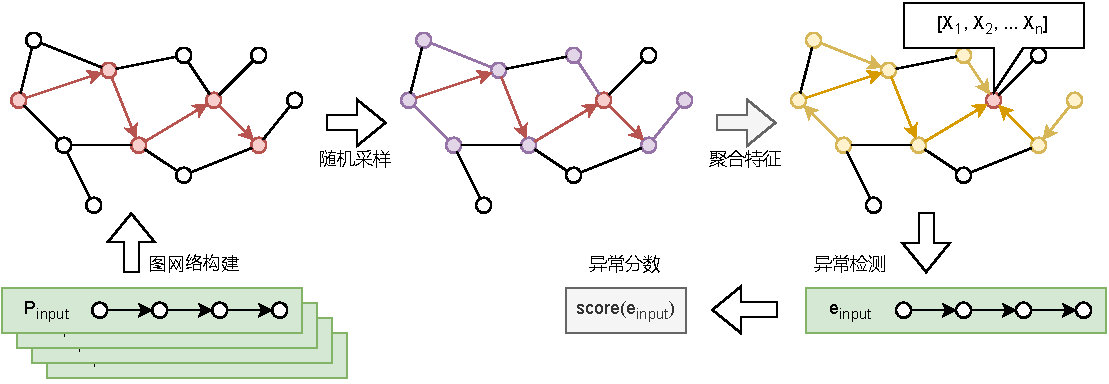
\includegraphics[width=\linewidth]{chapter/c4_images/c4_model.pdf}
    \caption{模型结构图}
    \label{c4_model}
\end{figure}

这一节的模型架构将以 GraphSAGE 模型为基础,通过对它的三个重要部分进行探讨,并针对广域网络的路由数据的特点,本研究从路径的角度出发分别提出对应的利用数据集中路径信息的方法。

如图 \ref{c4_model} 所示,本章提出的模型的结构包括了随机采样、聚合特征、异常检测三个部分,它的输入是一套网络路由数据集,首先输出对应数据集在图上的嵌入,最后通过异常检测输出对路由系统中路径更新的异常分数。

\begin{enumerate}
    \item 随机采样:该部分通过已知的路径信息优化随机采样的概率,从而实现有权重且权重基于路径信息的随机采样。
    \item 聚合特征:该部分通过引入路径带来的差异,对邻居间信息的聚合方式进行了调整,实现了基于路径权重的邻居聚合。
    \item 异常检测:该部分通过前序模型获得的嵌入,对比新路径的嵌入从而进行异常检测。
\end{enumerate}

\subsection{模型分析}

本文选取 GraphSAGE 作为模型的框架,是由于它具有以下特性:

\begin{enumerate}
    \item 训练数据通过采样获得。传统的图神经网络在面对网络路由等大规模的数据集上普遍存在性能不足的问题,GraphSAGE 通过采样子图的方式减小了需要计算的图网络矩阵尺寸,从而减少了性能开销。
    \item 聚合和采样函数具备调整空间。GraphSAGE 模型在框架上仅规定了前向传播的方法,具体的聚合和采样函数是模块化的,能够在节点层面上进行调整,这使得将路径因素引入到模型中是可行的。
\end{enumerate}

然而,GraphSAGE 模型非常依赖采样函数、聚合函数、损失函数的选取,在传统的 GraphSAGE 模型中路径是不存在的,这些函数仅会引入了节点连边的拓扑差异,在上述函数中直接采用现有方法不能利用数据集中的路径特征。因此,为了能够在路由数据集上针对性地提取特征,模型应当在这三个重要部分中体现出相应的权重差异,本研究通过在算法中引入路径因素,分别为三个部分设计了对应的改进方法。

\subsection{基于节点权重的随机采样}

大部分图网络中,图中的每个节点的度值是不一致的,为了提高模型性能,GraphSAGE 模型对于一般的图网络的通用做法\citing{hamilton2017inductive} 是为每个节点采样固定数量的邻居。而基于广域网络路由架构的性质而言,即使是在分布式网络中,广域网路由系统中的自治系统会在网络中对路由有着不同程度的控制力,即它们应当从/向不同尺度的节点获取/传递特征。

在图网络中,对节点在图网络中的控制力强度的度量方法通常是中心度,而对于在路由系统的嵌入任务而言,其中的介数中心度相比之下更具有统计意义,该方法能够将节点在最短路径中出现的频次,即介数中心度作为采样指标,从而在一定程度上反映自治系统对临接节点路由的控制能力,而这种控制能力的度量在实际场景中即对应其路由异常传播的规模。

为了验证这一结论,本研究针对节点的介数中心度的分布状况进行了实验分析。实验对来自 2022 年 10,11,12 三个月份的 RIPE RIS 数据样本按照第三章所述的基于拓扑的构图方式进行了图网络生成,以便排除对等路由的影响,随后对每一个自治系统计算了其对应的介数中心度,详细的统计结果如图 \ref{c4_node-centrality} 所示,为方便展示,横坐标轴已修改为通过对数的方式呈现。

\begin{figure}[h]
    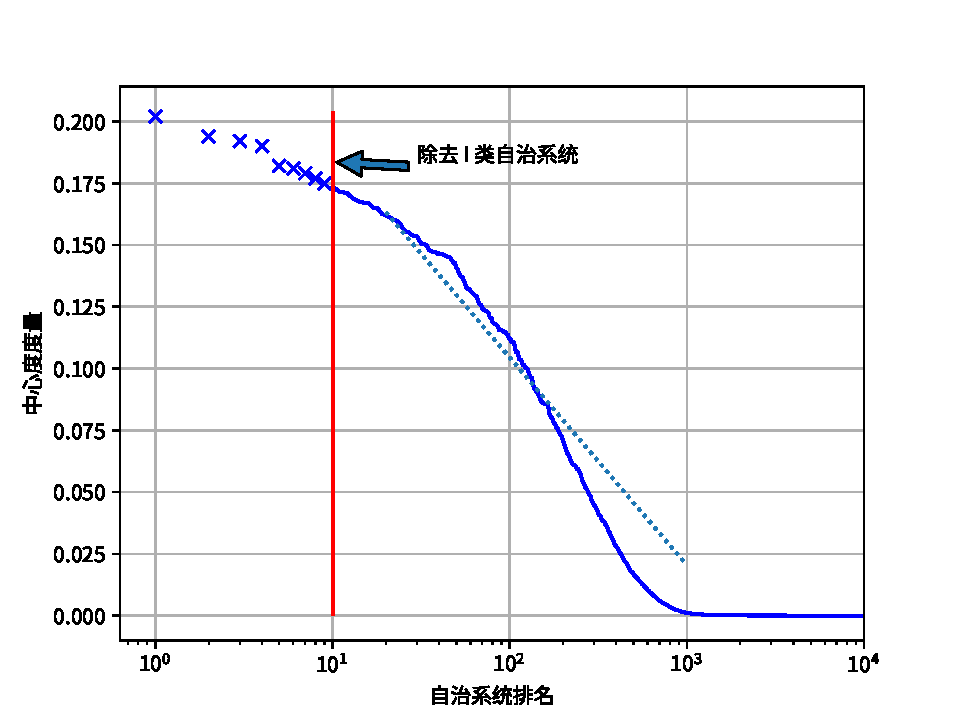
\includegraphics[width=0.8\linewidth]{chapter/c4_images/c4_node-centrality.pdf}
    \caption{RIPE 数据集中的介数中心度的分布状况}
    \label{c4_node-centrality}
\end{figure}

图 \ref{c4_node-centrality} 的结果可以反映出自治系统在中心度上的分布情况,由于 I 类自治系统自身根据定义具有很高的中心度,在去除了互联网所有 I 类自治系统(图中的红线部分右侧)后的图表趋势大致上在对数范围呈现线性下降的趋势(图中的蓝色虚线部分)。因而可以认为基于介数中心度的指标对节点进行采样和后续的特征聚合是可靠的。

因此,本章提出了如公式\ref{s3_sample_model}所示的采样模型:
\begin{equation} \label{s3_sample_model}
P_b(a) = \Sigma_{b, (a,b) \in E} \frac{\omega(a,b)}{\Sigma_{a} \omega(a,b)}, \omega(a,b) = 1 + \theta_{sample} \cdot \frac{N_{paths}^a(b)}{N_{paths}^a}
\end{equation}

其中 $\theta_{sample}$ 是一种权重值,通过它能够调整采样邻居数与其中心度的关联,当此值为 0 时,该模型退化至普通的固定采样模型。$N_{paths}^a(b)$ 是全部经由 a 节点的路径中同时经由 b 的路径数量,模型通过该式使得具有更多路径关联的邻居具有更大的采样概率。通过在原图网络上的 k 次迭代采样能够获得一个用于 k 层邻居聚合模型的子图。同时,为了限定采样规模,该采样过程由一个参数 $N_{sample}$ 控制,并决定对于一个节点而言的采样邻居数量。

根据此模型,在对邻居进行采样时将考虑到与邻居的共同路径比例,即更容易采样到具有更多公共路径的邻居信息。

\subsection{基于路由特征的邻居聚合}

一般而言,在 GraphSAGE 模型中一般使用均值聚合器方案\citing{hamilton2017inductive},即对相邻节点和本节点的上一层输出取均值,并据此进行线性变换,进而产生当前层的输出。具体的实现方式见公式\ref{graphsage_default_aggr}。
\begin{equation} \label{graphsage_default_aggr}
h^k_v \leftarrow \sigma(W \cdot MEAN(\{h_v^{k-1}\}\cup \{h^{k-1}_u, \forall u \in N(v)\}))
\end{equation}

在一般的图网络中,它能够对图节点的邻居特征起到很好的聚合效果。然而对于当前场景下的节点特征,由于存在路由路径相关的因素,对于一个自治系统即一个节点而言,它的相邻节点提供的路由路径是不一样的,聚合函数使用完全的均值函数将抹去邻居间由路径产生的的差异,从而没有利用上数据集中存在的路由特征。

为了聚合包含路径特征的相邻节点信息,本研究引入了一种新的聚合函数,定义如式\ref{graphsage_model_aggr}所示,它通过与路径相关的参数 $p(u)$ 控制的权重对邻居特征进行基于路径的聚合。
\begin{equation} \label{graphsage_model_aggr}
h^k_v \leftarrow \sigma(W \cdot MEAN(\{h_v^{k-1}\} \cup \{E\{p(u) \cdot h^{k-1}_u\}, \forall u \in N(v)\}))
\end{equation}

由于对相邻节点的相关统计量的操作均被包含在均值函数以内,它自身也具有类似均值聚合函数的结构,因而它满足聚合函数的对称性条件,即它能够确保模型能够被基于梯度的方式训练,并被应用在以任何可能顺序排列的临接节点的集合上。

根据以上的邻居聚合模型,一般的基于均值的聚合函数被加权平均的聚合函数替代,其中权值为经由路由更多的邻居节点。例如在如图 \ref{c4_nei-agg} 所示的采样子图中,传统的 GraphSAGE 模型没有考虑数据集的路径特征,在进行聚合时思路通常是对节点 $V_i$ 的所有邻居 $V_{nei}$ 及其高阶邻居赋予同样的权重进行求均值的处理;而在本模型中,由于存在路径的影响,节点 $V_i$ 在进行节点聚合时,将会相比于邻居节点 $V_b$ 和 $V_e$ 更多考虑来自邻居节点 $V_a$ 包含的特征信息,因为它们共享更多的与 $V_i$ 相关联的路由路径,这里也体现了本方法中基于路径特征的特点。

\begin{figure}[h]
    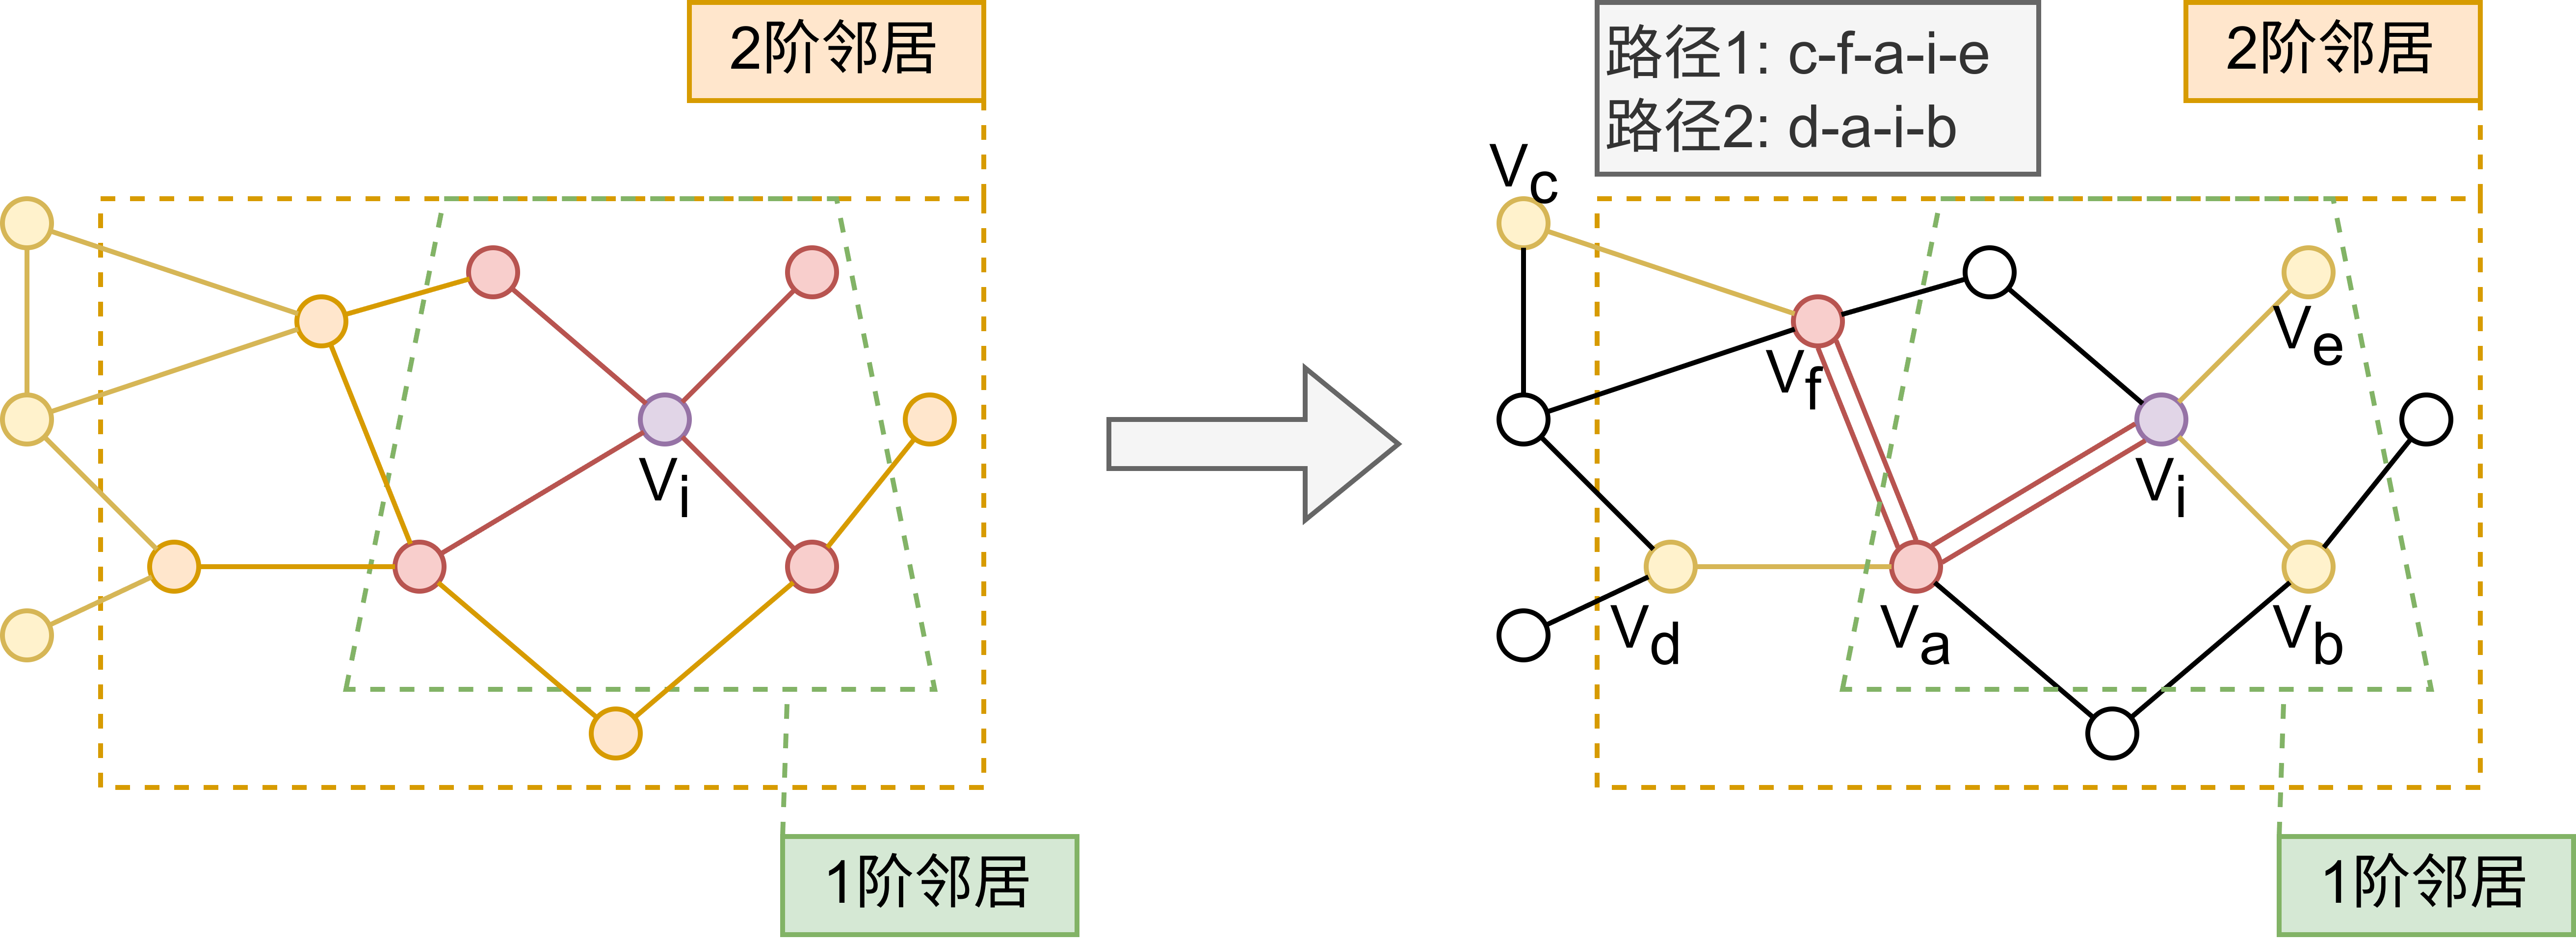
\includegraphics[width=0.9\linewidth]{chapter/c4_images/c4_nei-agg.png}
    \caption{邻居聚合方式的对比}
    \label{c4_nei-agg}
\end{figure}

\subsection{基于路由特征的损失设定}

基于与上一节相同的原理,本研究需要对基于图的无监督损失函数进行修正,它的原始定义如公式\ref{graphsage_default_loss}所示。
\begin{equation} \label{graphsage_default_loss}
J_G(Z_u) = -log(\sigma(z_u^{T}z_v)) - Q \cdot E_{v_n \sim P_n(v)}log(\sigma(-z_u^{T}z_v))
\end{equation}

它从当前节点的临接节点中采样对数损失,而从非临接节点中采样负的对数损失。该函数在 GraphSAGE 模型中被提出\citing{hamilton2017inductive},并被解释为一种实现在嵌入结果中相似嵌入节点更加接近的方法。

在本研究所述模型中,通过上述方式进行无监督的损失计算同样将抹去邻居间由路径产生的的差异,因而需要进行调整以适应存在路径特征的情形。

利用与上一节构造基于路径的聚合函数的方法可以设计一种损失函数,使得它能够可控地使得在同一条路径上的节点嵌入存在相似性,它的实现方式具体如公式\ref{graphsage_model_loss1}与公式\ref{graphsage_model_loss2}所示。
\begin{equation} \label{graphsage_model_loss1}
J(Z_u) = J_G(Z_u) + \theta_{loss} J_P(Z_u)
\end{equation}
\begin{equation} \label{graphsage_model_loss2}
J_P(Z_u) = -Q \cdot E_{v_n \sim P_{inpath}(v)}log(\sigma(z_u^{T}z_v)) -Q \cdot E_{v_n \sim P_{\sim inpath}(v)}log(\sigma(-z_u^{T}z_v))
\end{equation}

其中 $E_{v_n \sim P_{inpath}(v)}$ 表示在同一路径上的节点,即通过路径关联的节点;而 $E_{v_n \sim P_{\sim inpath}(v)}$ 表示不在同一路径上的节点,即互不通过路径关联的节点。

该损失公式通过结合图网络拓扑上的邻居损失 $J_G(Z_u)$ 和路径拓扑上的邻居损失 $J_P(Z_u)$,使得不仅相邻节点的嵌入更加相似,并且更多位于同一路径的节点(即路径意义上的邻居)应当在拓扑上更加相似。其中,$\theta_{loss}$ 控制了两种策略的比重,通过调整 $\theta_{loss}$ 的值能够使得节点更趋向与遵循基于路径的嵌入或是遵循基于网络拓扑的嵌入,而在具体损失的计算上依然沿用一般无监督学习所使用的对数损失函数,这在将模型运用于一些较少层次性的分布式网络中时能够适应其特点。

\subsection{异常检测方法}

在获得对应的节点嵌入后,对于需要检测的路由更新 $R_a$ 中路径的各节点 $V_i \in P_a \in R_a$ 获得对应的嵌入 ${e_i}$,并计算沿其路径相邻节点间的差异之和,此处使用如式\ref{negsim}所示的负对数相似度公式计算异常分数。
\begin{equation} \label{negsim}
D_a = \Sigma(||e_i - e_{i-1}||)
\end{equation}
在获得该值后即可通过设定一定的阈值以检测异常,即通过公式\ref{threshold}所描述的方法筛选大于 $\theta_{threshold}$ 的异常分数:
\begin{equation} \label{threshold}
p_{anomaly} = \{ \Sigma(||e_i - e_{i-1}||), v_i \in P_{input} \} \geq \theta_{threshold}
\end{equation}

然而,由于广域网络中的路由异常可能由正常操作导致,例如计划中的拓扑结构的改变,一般设置较低的阈值并对异常数值采取 top-k 的方式获得异常路由列表以供后续人工分析。